\section{Classification}

Nous avons décidé de comparer les pays fournis pour
les classer en trois catégories: les pays proches des pays
membres de l'UE, les pays proches des candidats à l'entrée
dans l'UE et les pays proches des pays non candidats non
membres de l'UE.

Nous avons pris comme critère les nouvelles technologies, à savoir
le taux d'utilisateurs d'Internet et le taux d'abonnés mobiles.

\subsection{{\sl Workflow}}

\begin{sidewaysfigure}[h!]
\begin{center}

    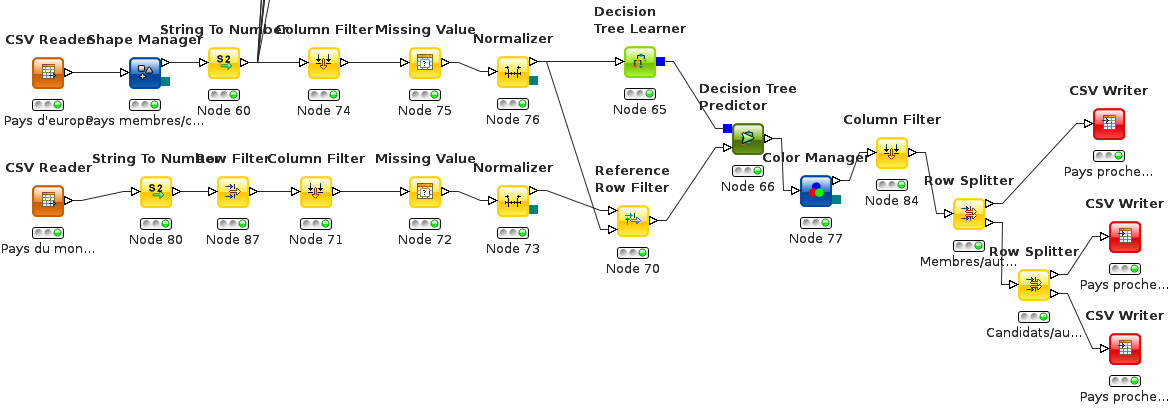
\includegraphics[width=22cm]{\PIXPATH/workflow_classif}

\end{center}
\end{sidewaysfigure}

\FloatBarrier

\subsection{Résultat}

\begin{center}
\rowcolors{1}{white}{gray!20}
\begin{longtable}{|c|c|c|}
\hline
{\bf Membre}&{\bf Candidat}&{\bf Non membre, non candidat}\\
\endhead
\hline
Antigua and Barbuda&Algeria&Bangladesh\\
\hline
Argentina&Angola&Benin\\
\hline
Aruba&Azerbaijan&Bhutan\\
\hline
Australia&Belize&Bolivia\\
\hline
Bahamas; The&Botswana&Burkina Faso\\
\hline
Bahrain&Cape Verde&Burundi\\
\hline
Brazil&China&Cambodia\\
\hline
Brunei Darussalam&Congo; Rep.&Cameroon\\
\hline
Canada&Ecuador&Central African Republic\\
\hline
Chile&El Salvador&Chad\\
\hline
Colombia&Equatorial Guinea&Comoros\\
\hline
Costa Rica&Fiji&Congo; Dem. Rep.\\
\hline
Dominican Republic&Gabon&Cote d'Ivoire\\
\hline
Faeroe Islands&Georgia&Cuba\\
\hline
French Polynesia&Indonesia&Egypt; Arab Rep.\\
\hline
Greenland&Kazakhstan&Eritrea\\
\hline
Hong Kong; China&Libya&Ethiopia\\
\hline
Iran; Islamic Rep.&Maldives&Gambia; The\\
\hline
Israel&Marshall Islands&Ghana\\
\hline
Jamaica&Micronesia; Fed. Sts.&Guinea\\
\hline
Japan&Namibia&Guinea-Bissau\\
\hline
Jordan&Paraguay&Haiti\\
\hline
Korea; Rep.&Samoa&Honduras\\
\hline
Kuwait&South Africa&India\\
\hline
Lebanon&Swaziland&Kenya\\
\hline
Liechtenstein&Tonga&Kiribati\\
\hline
Macao; China&Trinidad and Tobago&Korea; Dem. Rep.\\
\hline
Malaysia&Turkmenistan&Kyrgyz Republic\\
\hline
Mauritius&Vanuatu&Lao PDR\\
\hline
Mexico&&Lesotho\\
\hline
Morocco&&Liberia\\
\hline
New Caledonia&&Madagascar\\
\hline
New Zealand&&Malawi\\
\hline
Panama&&Mali\\
\hline
Peru&&Mauritania\\
\hline
Qatar&&Mongolia\\
\hline
Russian Federation&&Mozambique\\
\hline
Saudi Arabia&&Myanmar\\
\hline
Seychelles&&Nepal\\
\hline
Singapore&&Niger\\
\hline
St. Vincent and the Grenadines&&Nigeria\\
\hline
Syrian Arab Republic&&Oman\\
\hline
Thailand&&Pakistan\\
\hline
Tunisia&&Papua New Guinea\\
\hline
United Arab Emirates&&Philippines\\
\hline
United States&&Rwanda\\
\hline
Uruguay&&San Marino\\
\hline
Venezuela; RB&&Sao Tome and Principe\\
\hline
Vietnam&&Senegal\\
\hline
&&Sierra Leone\\
\hline
&&Solomon Islands\\
\hline
&&Somalia\\
\hline
&&Sri Lanka\\
\hline
&&Sudan\\
\hline
&&Tajikistan\\
\hline
&&Tanzania\\
\hline
&&Togo\\
\hline
&&Uganda\\
\hline
&&Uzbekistan\\
\hline
&&West Bank and Gaza\\
\hline
&&Zambia\\
\hline
&&Zimbabwe\\
\hline
\end{longtable}
\end{center}

